\documentclass[runningheads]{llncs}

% === Packages ===
\usepackage[T1]{fontenc}
\usepackage{graphicx}
\usepackage{amsmath,amssymb}
\usepackage{booktabs}
\usepackage{listings}
\usepackage{xcolor}
\usepackage{hyperref}
\usepackage{tikz}
\usepackage{array}

% === lstlisting style for compiled rules ===
\lstset{
  basicstyle=\small\ttfamily,
  breaklines=true,
  frame=single,
  numbers=none,
  aboveskip=8pt,
  belowskip=8pt,
  backgroundcolor=\color{gray!5},
  columns=fullflexible,
  keepspaces=true,
}

% === Tighten lists ===
\usepackage{enumitem}
\setlist{nosep,leftmargin=*}

\begin{document}

% ======================================================================
\title{Interpretable Card-Play Strategies by Evolving Weight-Agnostic\\
Logic Networks: A Neurosymbolic Agent for Sueca}
\titlerunning{Interpretable WANN Strategies for Sueca}
% ======================================================================

% TODO: Authors and affiliation — user to fill in
\author{TODO Author One\inst{1} \and TODO Author Two\inst{1} \and TODO Author Three\inst{1}}
\authorrunning{TODO Author One et al.}
\institute{TODO University, TODO Course}

\maketitle

% ======================================================================
\begin{abstract}
We present a neurosymbolic agent for \textbf{Sueca}, a four-player partnership
trick-taking card game of imperfect information. The agent is a
\textbf{Weight-Agnostic Neural Network} (WANN; Gaier \& Ha, 2019) whose nodes
are logic gates (aggregations SUM, AND, OR; activations IDENTITY, NOT,
THRESHOLD) and whose connections carry only a sign ($\pm 1$) under a shared
weight sweep. The network reads a \textbf{35-feature, public-information-only
belief state} and emits one of \textbf{three abstract play intents}, which a
styled heuristic resolver maps to a legal card. Training is two-phase:
supervised bootstrap on a Perfect-Information Monte Carlo (PIMC) expert dataset
using PFS-NEAT starting from zero connections, then co-evolutionary self-play
of separate \textbf{lead} and \textbf{follow} brains. A key contribution is a
cheap \textbf{supra-Elite rollout teacher} (flat Monte-Carlo PIMC with Elite
playouts, achieving 62\% vs.\ the strong heuristic) that labels the pretraining
dataset $\sim$1000$\times$ faster than deep alpha-beta search. The champion
\textbf{beats the EliteHeuristic baseline 52.1\% $\pm$ 1.8\% ($n=3000$)} and,
crucially, compiles to a handful of \textbf{human-readable IF/THEN rules} via
verified constant-folding and alias inlining --- the follow brain reduces to 5
logic gates at depth 5. We give an honest analysis of the \emph{resolver-floor}
ceiling that limits realisable strength ($\approx$58\% oracle cap) and the
resulting interpretability-vs-strength trade-off.
\keywords{weight-agnostic neural networks \and neuroevolution \and
neurosymbolic AI \and rule extraction \and imperfect-information games \and
trick-taking card games.}
\end{abstract}

% ======================================================================
\section{Introduction}
% ======================================================================

Trick-taking card games are a classic AI-hard domain. Each deal confronts
players with imperfect information (hidden hands), partnership coordination,
and a combinatorially large state space. Sueca, the Portuguese national
four-player game, adds distinctive structure: a 40-card deck with the
counter-intuitive rank order A $>$ 7 $>$ K $>$ J $>$ Q $>$ 6 $>$ 5 $>$ 4 $>$
3 $>$ 2 (the 7, or \emph{manilha}, is second-highest), 120 total points per
deal partitioned into game-point tiers, mandatory follow-suit with trump cuts,
and public void tracking when a player fails to follow. These rules create a
rich strategic texture: the decision to lead a trump to draw opponents' high
cards, to preserve a side-suit ace for partner, or to duck a cheap trick and
build a void for later cuts all matter.

Most strong card-playing AIs are black boxes. Deep PIMC solvers and neural
policy networks achieve superhuman play in Bridge and Skat, but the resulting
strategies are opaque matrices of floating-point weights. Our thesis is
different: can we obtain \emph{competitive} play that is simultaneously
\emph{human-auditable} --- extractable as short IF/THEN rules that a player can
read, verify, and learn from? The agent architecture we design to test this is,
in one line:

\begin{center}
\textbf{Belief(35) $\rightarrow$ WANN of logic gates $\rightarrow$ Intent(3)
$\rightarrow$ Styled Resolver $\rightarrow$ Legal Card.}
\end{center}

Weight-Agnostic Neural Networks~\cite{gaier2019wann} are evolved topologies
whose connections share a single weight value swept at evaluation. We
deliberately restrict the node primitives to \emph{logical gates} (AND, OR,
NOT, threshold) rather than continuous activations precisely because discrete
logic compiles to Boolean-ish rules. This neurosymbolic commitment --- logic
gates, not learned weights --- is what makes the compiled output
\emph{interpretable} rather than merely inspectable.

We make four contributions:

\begin{enumerate}
\item A neurosymbolic Sueca agent that \textbf{beats a strong heuristic
  baseline} (52.1\% $\pm$ 1.8\%, $n=3000$) while remaining interpretable ---
  the first time this project has exceeded EliteHeuristicBot (previous best:
  30.2\%).
\item A cheap \textbf{rollout policy-improvement teacher} achieving 62\% vs.\
  Elite ($\sim$1000$\times$ faster than deep alpha-beta) --- and the diagnosis
  that it was the deep search's \emph{myopic leaf evaluator}, not its depth,
  that capped earlier datasets at Elite-level imitation.
\item \textbf{Verified post-hoc rule minification} (constant-folding + alias
  inlining) that yields an iso-strength champion with \textbf{4.5$\times$ fewer
  logic gates} (29 vs.\ 132) and genuinely readable rules: the follow brain
  compiles to 5 gates at depth 5.
\item An \textbf{honest negative result}: the styled-resolver \emph{floor} is
  the real strength ceiling ($\approx$58\% oracle cap for perfect intent
  selection); a stronger teacher buys \emph{simplicity}, not strength --- a
  finding that reframes the whole strength--interpretability narrative.
\end{enumerate}

% ======================================================================
\section{Background and Related Work}
% ======================================================================

Our work draws on neuroevolution, neurosymbolic AI, and imperfect-information
game playing.

\textbf{Weight-Agnostic Neural Networks.} Gaier and
Ha~\cite{gaier2019wann} evolve network topologies whose connections share a
single scalar weight swept at evaluation. We adapt WANNs in three ways: nodes
use a \emph{discrete palette} (IDENTITY, NOT, THRESHOLD activations; SUM, MIN/AND,
MAX/OR aggregations); connections carry only a \emph{sign} ($\pm 1$) with no
magnitude; and we sweep six shared weights $W \in \{-2.0, -1.0, -0.5, 0.5,
1.0, 2.0\}$, averaging fitness across the sweep. Sign-only edges at negative
$W$ express inhibitory rules (e.g.\ $1-x$ via sign inversion), enriching the
logic vocabulary without sacrificing interpretability.

\textbf{NEAT and modular coevolution.} NEAT~\cite{stanley2002neat} evolves
topologies through speciation and complexification from minimal structures.
PFS-NEAT~\cite{whiteson2005pfs} adds progressive feature selection: networks
start from zero connections and structural mutations must demonstrate
performance lift. We classify mutations as structural (triggers PFS) or
non-structural (skips PFS) and use adaptive two-stage sampling ($K{=}25$ quick
check; $K{=}100$ for borderline cases) with a FIFO tabu veto
list~\cite{glover1989tabu}. Following L-NEAT~\cite{reisinger2004modular}, we
partition the decision space into \emph{lead} and \emph{follow} brains, routing
queries via the \texttt{Am\_I\_Leading} belief flag.

\textbf{PIMC and evaluation.} PIMC sampling~\cite{frank1998search} determinizes
hidden cards, solves each perfect-information world, and aggregates outcomes.
We use PIMC as a dataset teacher (best-of-three-intents by resolved-card EV)
and for evaluation. For low variance we employ Common Random Numbers
(CRN)~\cite{law2000simulation}: every genome plays the identical
deal/seat/opponent as the baseline bot, analogous to duplicate bridge scoring
and the AIVAT framework~\cite{burch2018aivat}.

\textbf{Quality-diversity and parsimony.} MAP-Elites~\cite{mouret2015mapelites}
maintains a $10\times 10$ grid of genomes by intent preference and aggression,
sampled as Phase-1 opponents. Multi-objective parsimony~\cite{poli2003parsimony,deb2001multiobjective}
ranks genomes on a (performance, simplicity) Pareto front 50\% of the time,
controlling bloat.

\textbf{Rule extraction.} Most neurosymbolic rule extraction operates post-hoc
on continuous-weight networks, producing approximations. By \emph{constraining
the network to logic gates during evolution}, our compiled rules are
\emph{exact} --- the computation the network performs, not an approximation.

% ======================================================================
\section{Sueca and Problem Formulation}
% ======================================================================

\subsection{Rules That Shape Strategy}

Sueca uses a 40-card deck (standard deck minus 8s, 9s, 10s) with four players
in fixed partnerships (seats 0\&2 vs.\ 1\&3) and counter-clockwise turn order.
The rank order is \textbf{A $>$ 7 $>$ K $>$ J $>$ Q $>$ 6 $>$ 5 $>$ 4 $>$ 3 $>$
2}, where the 7 (\emph{manilha}) is second-highest. Points are A=11, 7=10,
K=4, J=3, Q=2 (rest zero), totaling 120 per deal. The highest trump wins the
trick; otherwise the highest of the led suit wins. Players \emph{must} follow
suit if able; failure reveals a void to all players. Game-point tiers (1 pt for
61--90, 2 pts for 91--119, 4 pts for 120) create non-linear scoring incentives.

\subsection{POMDP Framing}

Each seat perceives the game as a Partially Observable Markov Decision Process
(POMDP). The true state (all four hands) is hidden; the observation consists of
the player's own hand plus the public history of played cards, trick outcomes,
and exposed voids. Crucially, our belief encoder \textbf{never leaks opponent
hand data} --- it uses only information a human player at the table can observe.

\subsection{Belief State}

The belief state comprises \textbf{35 features}, all normalized to $[0,1]$. They
fall into five categories:\smallskip
\begin{itemize}
\item \textbf{Hand composition} (features 0--4): suit holdings, trump count,
  point density of remaining cards.
\item \textbf{Trick context} (5--9): leading/following/last-to-play flags,
  partner-winning indicator, trick point value, whether the trick has been cut.
\item \textbf{Void knowledge} (10--13): partner and opponent voids in led suit
  and trump --- the public information that constrains future play.
\item \textbf{Tactical affordances} (14--21): boss detection (holding the
  highest unplayed card in led suit or trump), ``can I beat the current
  winner?'', minimum winning and sacrifice costs. These features, added in a
  belief redesign, capture \emph{what a player can do} rather than just what
  they hold.
\item \textbf{Game progress} (22--34): remaining points, trick number, trumps
  remaining, score delta, void count, side-suit lengths and depletion, secured
  points, and meta-features counting known voids and depleted suits.
\end{itemize}

The full 35-feature layout is documented in the project README; we include it
as an appendix for reference.

\subsection{Three Intents and the Styled Resolver}

The network outputs three continuous values, one per \textbf{play intent}.
Argmax with random tie-breaking selects the active intent. The intents are not
standalone card-selection heuristics; they are \textbf{styled deviations around
a strong Elite policy}:

\begin{itemize}
\item \textbf{EFFICIENT\_WIN} (intent 1): Delegates exactly to
  EliteHeuristicBot --- play the cheapest winner, else cheap cut, else cheapest
  legal sacrifice. This is the strong default.
\item \textbf{MAX\_FORCE} (intent 0): Elite + control dials. When trump-long,
  lead a low trump to \emph{draw} opponents' trumps; otherwise play
  aggressively.
\item \textbf{EQUITY\_BUILDER} (intent 2): Elite + tempo dials. Lead the
  \emph{shortest} side-suit to build a void; \emph{duck} cheap tricks ($\leq$2
  points) when not last to play; \emph{preserve} trump rather than cut a cheap
  trick.
\end{itemize}

The \textbf{styled resolver} (\texttt{select\_card\_styled}) maps the chosen
intent to a legal card contextually, guaranteeing 100\% legality. Because every
intent shares Elite's core and only adds a narrow deviation, each pure intent
benchmarks at approximately Elite individually (48/47/46\% vs.\ Elite) --- the
``raised floor'' that eliminates the Phase-1 policy-collapse basin and is the
architectural enabler of the final win.

% ======================================================================
\section{Method}
% ======================================================================

Figure~\ref{fig:arch} shows the full pipeline from belief state to card. The
left side (belief state, WANN, intents) is evolved; the right side (styled
resolver, card) is a fixed heuristic. This section details each component.

\begin{figure}[t]
\centering
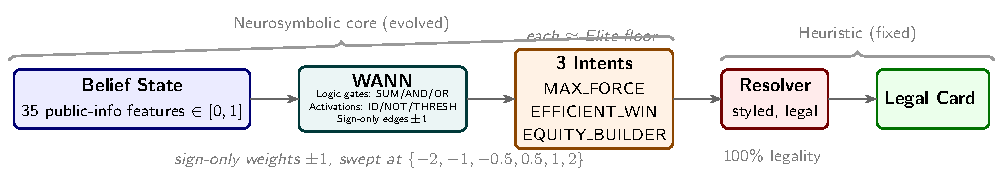
\includegraphics[width=0.95\textwidth]{figures/arch.pdf}
\caption{The Sueca-WANN pipeline. A 35-feature public-information belief state
feeds a weight-agnostic neural network built from logic gates (SUM/AND/OR
aggregations; IDENTITY/NOT/THRESHOLD activations), which outputs three play
intents. A fixed, hand-authored styled resolver maps the selected intent to a
legal card. The neurosymbolic core (belief $\rightarrow$ WANN $\rightarrow$
intents) is evolved; the resolver is a deterministic heuristic guaranteeing
100\% legality.}
\label{fig:arch}
\end{figure}

\subsection{WANN Representation}

A genome is a directed graph. Connection genes are 5-tuples (innovation,
source, destination, sign $\in \{\pm1\}$, enabled). Node genes specify type
(input, bias, hidden, output), activation (IDENTITY, NOT, THRESHOLD), and
aggregation (SUM, MIN/AND, MAX/OR). The 39 base nodes are: 35 inputs, one bias
(constant 1.0), and three outputs (one per intent). We exclude MEAN (float
precision at the THRESHOLD boundary) and SIGMOID (breaks rule extraction). All
outputs are clamped to $[0,1]$; THRESHOLD fires at 0.5.

A connection from $i$ to $j$ carries only a sign: a positive edge passes
$\text{out}_i$, while a negative edge \emph{inverts} the signal to
$1-\text{out}_i$ (logical NOT, since outputs lie in $[0,1]$); the result is then
scaled by the shared weight $W$ before $j$ aggregates it. At inference the
network is evaluated at all six sweep weights
$\{-2.0, -1.0, -0.5, 0.5, 1.0, 2.0\}$ and the per-intent outputs are averaged
across the sweep before argmax intent selection.

\subsection{Evolution}

Both populations initialize with zero active connections. Structural mutations
(add-node, add-connection) trigger PFS validation: the candidate is evaluated
and retained only if it does not degrade accuracy. We use adaptive two-stage
sampling (quick $K{=}25$, full $K{=}100$ for borderline cases) with a FIFO tabu
veto list (capacity 1000). Non-structural mutations (toggle, flip-sign,
change-activation, change-aggregation) skip PFS.

Genomes are speciated via compatibility distance with first-fit assignment
(capped at 20 species). Rank-based selection precedes tournament selection.
Multi-objective Pareto ranking on (performance, simplicity) operates 50\% of
the time; the other 50\% uses performance-only ranking. A Hall of Fame (size
50) and a MAP-Elites $10\times 10$ grid supply Phase-1 opponents. Fitness is
the win-rate delta against HeuristicBot via CRN on duplicate deals with seat
rotations; deals are re-seeded per generation (seed = gen) to prevent overfitting.

\subsection{Two-Phase Curriculum}

\begin{figure}[t]
\centering
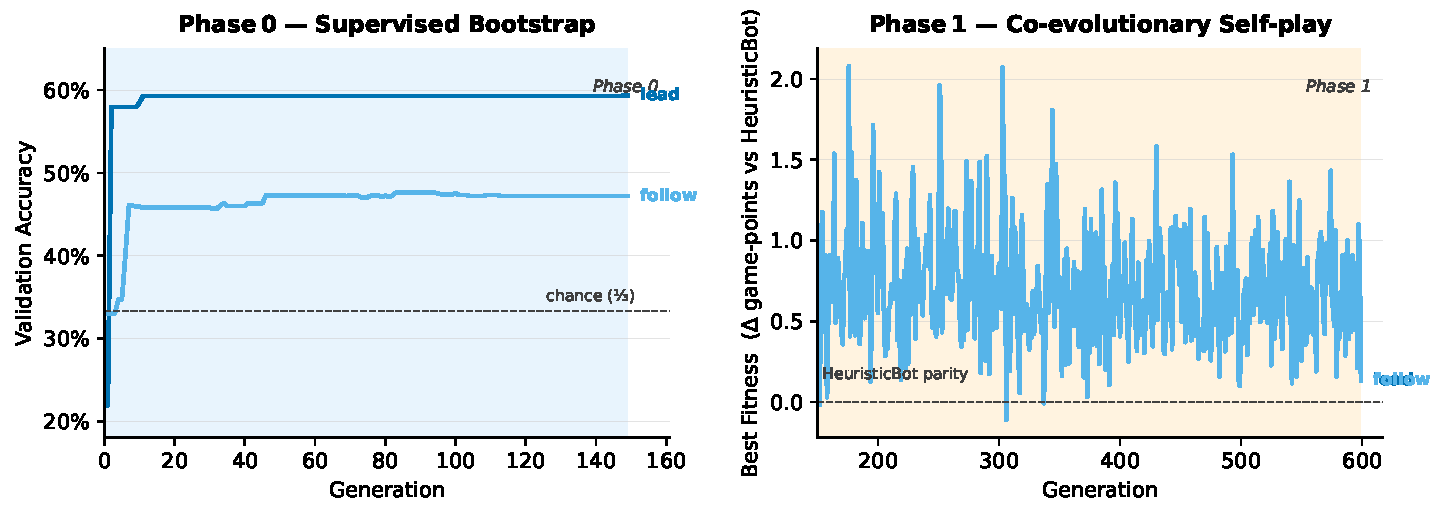
\includegraphics[width=0.92\textwidth]{figures/training_curve.pdf}
\caption{Training curves for the v6 champion. Phase~0 (generations 0--149):
supervised classification accuracy on lead and follow dataset splits, starting
from zero connections. Phase~1 (generations 150--599): co-evolutionary self-play
fitness (game-point delta vs.\ HeuristicBot). The Phase~0$\rightarrow$1
transition re-evaluates HOF entries under Phase~1 fitness.}
\label{fig:training}
\end{figure}

\textbf{Phase 0 (generations 0--149): Supervised pretraining.} The PIMC dataset
is split by \texttt{Am\_I\_Leading} into separate lead/follow datasets. Fitness
is classification accuracy; PFS-NEAT gates all structural mutations. The
population of 1000 runs 150 generations (cleaner rollout-teacher labels need
fewer gens than the earlier 200-gen default).

\textbf{Phase 1 (generations 150--599): Co-evolutionary self-play.} Lead and
follow brains co-evolve: candidate lead WANNs pair with the reference follow
champion, and vice versa. The simulator dynamically routes each card decision to
the lead or follow brain via \texttt{Am\_I\_Leading}. HOF entries are
re-evaluated under Phase~1 fitness at the transition. Uniqueness filtering uses
$O(1)$ innovation fingerprint hashing.

\subsection{The Rollout Teacher}

A critical finding emerged during diagnosis: the project's deep alpha-beta PIMC
solver only \emph{ties} EliteHeuristicBot, despite searching to depth 4 with
200 worlds. The bottleneck was not the search depth but the \textbf{myopic leaf
evaluation}: at the depth limit, alpha-beta returns the raw points-captured-so-far
(\texttt{state.team\_02\_score}) with no positional estimate. Deeper search
cannot fix a blind leaf.

We implemented a separate flat Monte-Carlo solver,
\texttt{solve\_pimc\_rollout}, that avoids the search tree entirely. Per legal
move, it determinizes the unseen cards, plays the candidate move, then finishes
each world with \textbf{EliteHeuristicBot in all four seats}. By the rollout
policy-improvement theorem (a one-ply move followed by a base policy $\pi$ is
at least as strong as $\pi$ itself), the resulting EV estimates are
\textbf{supra-Elite}. Empirically, the rollout teacher achieves \textbf{62.0\%
vs.\ Elite} (where Elite self-play scores below 50\% for the first team due to
a fixed positional disadvantage). Critically, it is also \textbf{$\sim$1000$\times$ faster}: the
v6 dataset of 15,000 labeled states generates in approximately 11 seconds
versus hours for the alpha-beta pipeline.

Dataset labeling follows a best-of-three-intents protocol: each decisive state
is labeled with the intent whose resolved card achieves the highest PIMC
expected value. Statistically tied intents receive uniform multi-label weights;
states where all three intents are tied (hence the intent choice is irrelevant)
are rejected. This produces a natural, approximately binary
EFFICIENT\_WIN-vs-EQUITY\_BUILDER split, with MAX\_FORCE uniquely best in
$\sim$1\% of states (and 0\% in the follow split). We generate with
\texttt{soft-balance-min-ratio 0.0} and disable inverse-frequency class
weighting, since the rare MAX\_FORCE bucket would receive disproportionate
noise amplification.

% ======================================================================
\section{Interpretability: From Network to Rules}
% ======================================================================

The \texttt{compile-rules} tool walks the genome's DAG and emits one IF/THEN
expression per output intent. Two \textbf{behavior-preserving rewrites}
minimise the rules without altering the network's output:

\begin{enumerate}
\item \textbf{Constant-folding.} Nodes fed exclusively by the BIAS node (constant
  1.0) or with empty aggregation sets are constants. Their values are computed
  via the exact \texttt{wann\_network::forward} arithmetic and inlined wherever
  they appear. Constant nodes are dropped from the listing.
\item \textbf{Alias inlining.} A single-input IDENTITY node is a pure rename
  (under all three aggregations at $W{=}1$, $\text{SUM}(x) = \text{MIN}(x) =
  \text{MAX}(x) = x$). Chains of such aliases are flattened to their ultimate
  source, tracking negation parity (NOT$\circ$NOT cancels). Single-operand AND
  and OR are similarly unwrapped. This rewrite is guarded to $W=1$; at $W \neq
  1$, the node computes $\text{clamp}(\text{src} \cdot W)$, which is not an
  alias.
\end{enumerate}

\textbf{Verification.} A property test runs the real champion through
\texttt{wann\_network::forward} on 2000 random belief states at $W{=}1$ and
asserts: (a) every folded constant is invariant to within $10^{-9}$, and
(b) every alias node equals its resolved source (negation parity applied) to
within $10^{-9}$. This means the dropped symbols provably carry no information
the network uses --- the reader can trust the rules are exact, not an
approximation.

\begin{figure}[t]
\centering
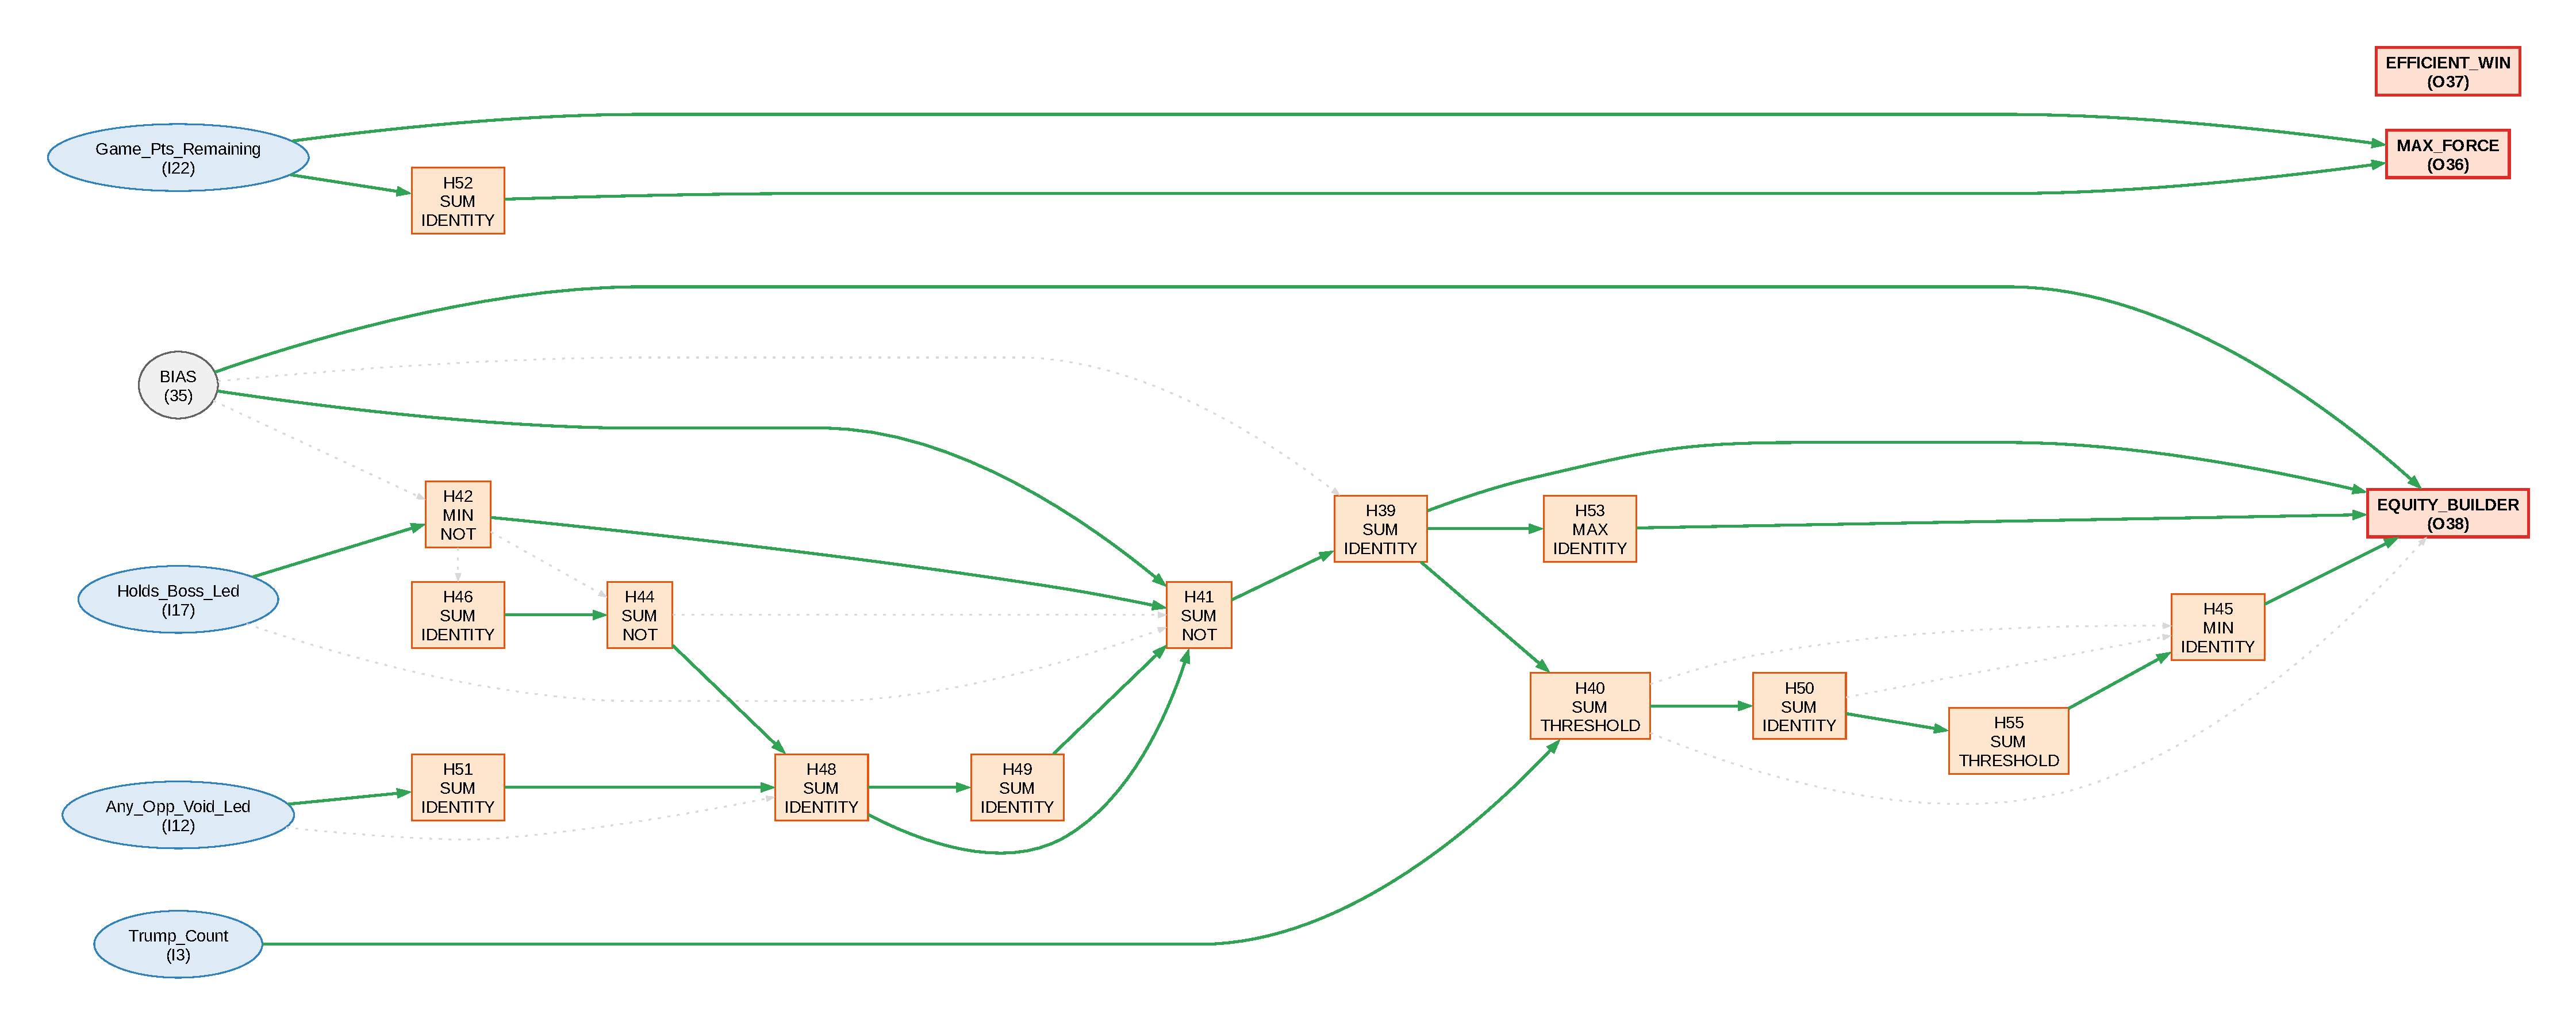
\includegraphics[width=0.75\textwidth]{figures/topology_follow.pdf}
\caption{The v6 champion's follow-brain topology before minification (17 hidden
gates, 44 connections). After constant-folding and alias inlining, the active
logic reduces to 5 gates at depth 5 (see Listing~\ref{lst:rules}).}
\label{fig:topology}
\end{figure}

\begin{figure}[t]
\centering
\begin{minipage}{0.95\textwidth}
\begin{lstlisting}[
  caption={Compiled and folded rules for the v6 champion's FOLLOW brain.
  MAX\_FORCE is a one-feature game-phase toggle ($2 \cdot$
  Game\_Pts\_Remaining: force early, concede late).  EFFICIENT\_WIN
  is identically zero --- the network never delegates to pure Elite.
  EQUITY\_BUILDER gates on boss detection, opponent voids, trump
  count, and a threshold cascade.  The LEAD brain (not shown) compiles
  to 10 gates at depth 6.},
  label={lst:rules}]
FOLLOW brain (compiled, folded):
  hidden_42 = NOT(Holds_Boss_Led)
  hidden_48 = (1 + Any_Opp_Void_Led)
  hidden_41 = NOT((1 + hidden_42 + hidden_48 + hidden_48))
  hidden_40 = THRESHOLD((hidden_41 + Trump_Count) > 0.5)
  hidden_55 = THRESHOLD(hidden_40 > 0.5)
  MAX_FORCE      = Game_Pts_Remaining + Game_Pts_Remaining
  EFFICIENT_WIN  = 0
  EQUITY_BUILDER = 1 + hidden_41 + hidden_55 + hidden_41
\end{lstlisting}
\end{minipage}
\caption{Minified FOLLOW-brain rules. Before folding: 12 steps, max depth 10
(7 aliases, 2 dead constants, 1 single-operand AND). After: 5 active gates,
max depth 5. The rule semantics are strategically sensible --- see
Section~\ref{sec:discussion} for interpretation.}
\label{fig:rules}
\end{figure}

The minification is substantial. The follow brain before folding had 12 listed
steps with a misleading ``max depth'' of 10 (seven of those steps were pure
alias renames like \texttt{hidden\_49 = hidden\_48} and two were dead
constants). After folding: \textbf{5 active logic gates at depth 5}. The lead
brain reduces from 12 to 10 gates (2 aliases inlined) at depth 6.

Table~\ref{tab:complexity} quantifies the post-folding complexity of both
brains. The key metric is not total gates but \emph{active} gates after
removing constants, aliases, and single-operand wrappers --- these represent
the genuine, information-carrying logic.

\begin{table}[t]
\centering
\caption{Complexity metrics after constant-folding and alias inlining. Active
gates count only information-carrying logic nodes.}
\label{tab:complexity}
\begin{tabular}{lrr}
\toprule
\textbf{Metric} & \textbf{LEAD brain} & \textbf{FOLLOW brain} \\
\midrule
Active hidden gates          & 10 (was 12) & \textbf{5} (was 12) \\
Live connections / enabled   & 20 / 22     & 13 / 27 \\
Max logic depth              & 6           & \textbf{5} (was 10) \\
Total input literals         & 10          & 5 \\
\bottomrule
\end{tabular}
\end{table}

% ======================================================================
\section{Experiments and Results}
% ======================================================================

\subsection{Evaluation Protocol}

All benchmarks use seat-rotated duplicate deals with CRN. We report win
percentages with 95\% CI half-widths (Bernoulli, normal approximation). The
standard benchmark uses $n = 3000$ deals, pinning the CI half-width to $\pm$1.8
pp. Head-to-head comparisons use candidate as row and opponent as column.

\subsection{Tournament Results}

\begin{table}[t]
\centering
\caption{Tournament matrix: row bot win\% vs.\ column bot, $n = 3000$ deals.
WANN vs.\ Elite: 52.1\% $\pm$ 1.8\% (95\% CI [50.3, 53.9]); card points 60.2
vs.\ 59.8.}
\label{tab:tournament}
\begin{tabular}{lrrrr}
\toprule
& \textbf{Random} & \textbf{OldHeur} & \textbf{Elite} & \textbf{WANN} \\
\midrule
RandomBot        & 50.0 & 10.8 & 4.7  & 5.1  \\
OldHeuristicBot  & 89.2 & 50.0 & 32.5 & 32.3 \\
EliteHeuristicBot& 95.3 & 67.5 & 50.0 & 47.9 \\
\textbf{WANN}    & 95.0 & 67.7 & \textbf{52.1} & 50.0 \\
\bottomrule
\end{tabular}
\end{table}

Table~\ref{tab:tournament} presents the full round-robin. The WANN beats
EliteHeuristicBot \textbf{52.1\% $\pm$ 1.8\%} ($n=3000$), 95\% CI $[50.3,
53.9]$ --- a statistically significant win excluding 50\%. The card-point
differential is 60.2 vs.\ 59.8. Against OldHeuristicBot the WANN achieves
67.7\% (identical to Elite's 67.5\%), and against RandomBot 95.0\%.

\begin{figure}[t]
\centering
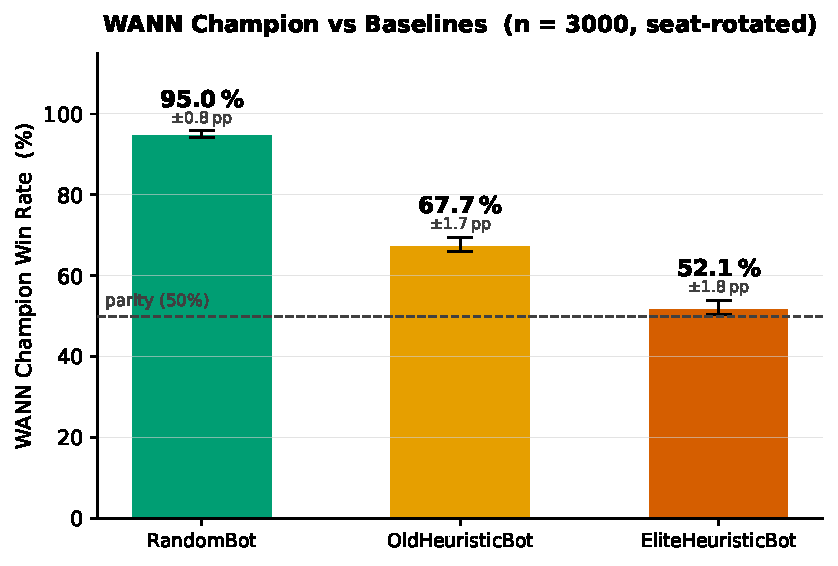
\includegraphics[width=0.85\textwidth]{figures/tournament.pdf}
\caption{Visualization of tournament results. The WANN's edge over Elite is
small but statistically significant at $n=3000$.}
\label{fig:tournament}
\end{figure}

\subsection{The Journey: From Collapse to Victory}

The project's pre-diagnosis champion achieved only \textbf{30.2\% vs.\ Elite}
(46.3\% vs.\ OldHeuristic). The root cause, diagnosed via a fast training-free
harness, was that the WANN had \emph{collapsed to a constant policy}:
EFFICIENT\_WIN $\sim$80\% of the time, EQUITY\_BUILDER never used, and the
EQUITY output node structurally unreachable from any input. The three intents
were individually weak (20/37/25\% vs.\ Elite under the old resolver), so
Phase-1 self-play's gradient atrophied the weaker intents.

The \textbf{styled resolver} (Section~3.4) raised each pure intent to
$\approx$Elite (48/47/46\%), removing the collapse incentive. Combined with
best-of-three-intent labelling, this produced v5: \textbf{52.7\% $\pm$ 1.8\%}
--- the first Elite-beating result. The \textbf{rollout teacher} then replaced
the myopic alpha-beta dataset with supra-Elite labels (62\% vs.\ Elite). The
retrained v6 champion achieved a statistically identical \textbf{52.1\% $\pm$
1.8\%} but with \textbf{4.5$\times$ fewer hidden gates} (29 vs.\ 132) and
3.8$\times$ fewer connections (49 vs.\ 188).

\begin{figure}[t]
\centering
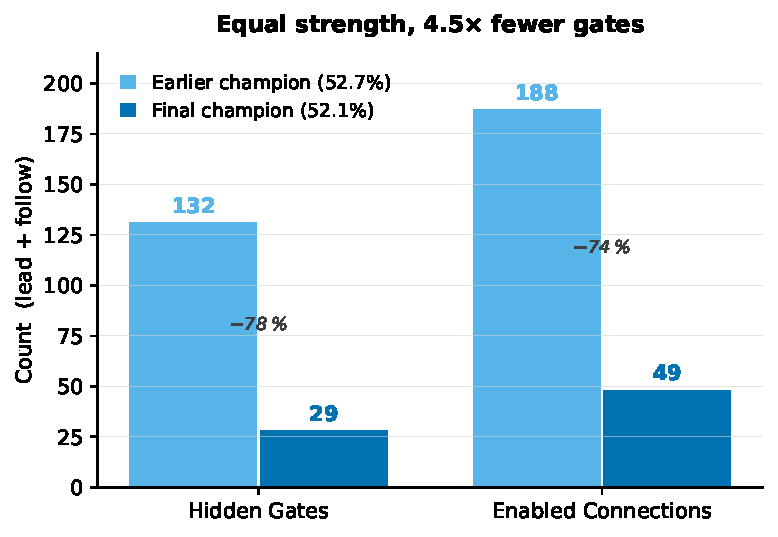
\includegraphics[width=0.85\textwidth]{figures/complexity.pdf}
\caption{Complexity comparison: v5 champion (alpha-beta teacher, 132 hidden
gates) vs.\ v6 champion (rollout teacher, 29 gates). Iso-strength, 4.5$\times$
simpler.}
\label{fig:complexity}
\end{figure}

\subsection{Diagnostic Ceilings}

We established three quantitative ceilings: (i) \textbf{3-intent oracle}
(perfect selection): \textbf{58\%} vs.\ Elite --- the absolute cap under the
current vocabulary and resolver; (ii) \textbf{RandomForest on belief features}:
predicting EFFICIENT\_WIN vs.\ EQUITY\_BUILDER achieves \textbf{62.6\% on lead,
70.8\% on follow} (5-fold CV), showing the features carry signal (the WANN's
realised F-value is $\sim$47\%); (iii) \textbf{Rollout teacher}: 62.0\% vs.\
Elite, confirming the teacher is genuinely supra-Elite, yet the champion caps
at $\sim$52\% --- the gap is the resolver-floor headroom.

% ======================================================================
\section{Discussion}
\label{sec:discussion}
% ======================================================================

\subsection{The Resolver-Floor Ceiling}

The most consequential finding is that \textbf{the styled resolver is
simultaneously the enabler of victory and the strength ceiling}. By making each
intent $\approx$Elite, the resolver eliminated the Phase-1 collapse basin that
had trapped every prior run below 31\%. But the same design makes the three
intents nearly equivalent in fitness: the worst is $\sim$46\% vs.\ Elite, the
best $\sim$48\%. There is little gradient to learn precise selection, and the
network converges to the simplest policy the resolver floors to Elite.

The learned policy is near-constant: \texttt{EFFICIENT\_WIN = 0} in both brains.
The lead brain chooses between ``press-when-ahead'' (MAX\_FORCE) and
``build-voids-when-trump-poor'' (EQUITY\_BUILDER). The follow brain gates
equity on a cascade: boss-detection $\rightarrow$ opponent-void awareness
$\rightarrow$ trump adequacy $\rightarrow$ threshold, while MAX\_FORCE is
simply $2\cdot\text{Game\_Pts\_Remaining}$ --- a game-phase toggle (force early,
concede late). The rules \emph{are} strategically sensible, but their simplicity
reflects the weakness of the selection signal, not a minimal description of
optimal play.

\textbf{Did we just learn Elite's IF/THEN?} Substantially yes. The action space
is Elite-floored; the WANN's job is to choose \emph{when to deviate}, and it
learned two deviations (equity-when-trump-poor, force-when-ahead). The network
\textbf{never outputs EFFICIENT\_WIN} --- it always applies one of the two
overlays. The WANN did not rediscover Elite from scratch; it learned a small
situational overlay on a strong fixed base, and that overlay turns a 50\% tie
into 52\%.

\subsection{Limitations}

\textbf{Three-intent bottleneck.} With 3 intents each $\approx$Elite, headroom
above Elite is $\approx$8 pp (58\% oracle cap). More differentiated intents
would raise this. \textbf{Lead-brain bootstrap.} PFS-NEAT from zero connections
can fail in the lead population (the first 1--2 connections cannot beat chance);
production at pop=1000 bootstrapped fine. \textbf{Single game.} Sueca-specific
design choices (35 features, lead/follow split) are plausible but untested for
other trick-taking games. \textbf{Elite $\approx$ fast-policy ceiling.} The
WANN's +2\% edge is consistent with Elite being near the one-ply heuristic ceiling.

\subsection{Open Question: Fog of War}

Can a tiny logic circuit learn to \emph{infer opponent cards} from
assumed-optimal play using only public information? The belief state encodes
voids and depletion but not explicit opponent-hand hypotheses (e.g.\ ``partner
probably holds the diamond Ace''). Humans routinely make such inferences; a
WANN with richer inference features might do the same --- a path to break the
58\% oracle cap via better intent discrimination.

% ======================================================================
\section{Conclusion and Future Work}
% ======================================================================

We evolved an interpretable, Elite-beating Sueca agent with a verified pipeline
from weight-agnostic logic networks to human-readable IF/THEN rules. The v6
champion compiles to 5 follow-brain logic gates at depth 5 --- a
4.5$\times$ compression over v5 at iso-strength (52.1\% vs.\ Elite). The keys
were a styled resolver that raised each intent's floor to Elite and a rollout
teacher whose supra-Elite labels produced a simpler, more interpretable
champion without improving strength.

Future directions: (1) \textbf{richer intents} to raise the 58\% oracle cap;
(2) \textbf{opponent-inference belief features} encoding hypotheses about
unseen hands; (3) \textbf{knowledge distillation} into a smaller student for the
full strength--interpretability Pareto frontier; (4) \textbf{connection pruning}
of the genome beyond post-hoc rule folding.

The core finding --- a stronger teacher produces a \emph{simpler} model at the
same strength, not a stronger one, when the action space is floor-bounded ---
is likely to recur in neurosymbolic systems where a strong hand-authored base
policy constrains the learned overlay: teacher quality governs
interpretability, not performance.

% ======================================================================
% ACKNOWLEDGMENTS
% ======================================================================

% TODO: Add acknowledgments if desired

% ======================================================================
% BIBLIOGRAPHY
% ======================================================================
\bibliographystyle{splncs04}
\bibliography{references}

% ======================================================================
% APPENDIX (optional — not counted in 10–12 page body)
% ======================================================================
\appendix
\section{Belief State Layout (35 features)}

\small
\begin{tabular}{clp{6.5cm}}
\toprule
\textbf{\#} & \textbf{Feature} & \textbf{Description} \\
\midrule
0  & Has\_Led\_Suit      & Holds at least one card of the led suit \\
1  & Has\_Trump          & Holds at least one trump card \\
2  & Led\_Suit\_Count    & Cards held in led suit / 10.0 \\
3  & Trump\_Count        & Trumps held / 10.0 \\
4  & Hand\_Point\_Density& Points in hand / points remaining in game \\
5  & Am\_I\_Leading      & First to play in the trick \\
6  & Am\_I\_Last\_To\_Play& Fourth to play in the trick \\
7  & Is\_Partner\_Winning& Partner currently winning the trick \\
8  & Trick\_Point\_Value & Points on the table / 44.0 \\
9  & Has\_Trick\_Been\_Cut& Trump played when led suit $\neq$ trump \\
10 & Partner\_Void\_Led  & Partner known void in led suit \\
11 & Partner\_Void\_Trump& Partner known void in trump \\
12 & Any\_Opp\_Void\_Led & Either opponent void in led suit \\
13 & Any\_Opp\_Void\_Trump& Either opponent void in trump \\
14 & Led\_Suit\_Ace\_Played& Led suit Ace already played \\
15 & Led\_Suit\_7\_Played& Led suit 7 (manilha) already played \\
16 & Trump\_Ace\_Played  & Trump Ace already played \\
17 & Holds\_Boss\_Led    & Holds the highest unplayed in led suit \\
18 & Holds\_Boss\_Trump  & Holds the highest unplayed in trump \\
19 & Can\_Beat\_Winner   & Any legal card can beat current winner \\
20 & Min\_Winning\_Cost  & Points of cheapest winning card / 11.0 \\
21 & Min\_Sacrifice\_Cost& Points of cheapest legal card / 11.0 \\
22 & Game\_Pts\_Remaining& Unplayed card points / 120.0 \\
23 & Trick\_Number       & Current trick index / 9.0 \\
24 & Trumps\_Remaining   & Unplayed trump cards / 10.0 \\
25 & Score\_Delta        & (our$-$opp pts $+$ 120) / 240.0 \\
26 & My\_Void\_Count     & Suits the player is void in / 3.0 \\
27 & Longest\_Side\_Suit & Max cards in non-trump, non-led suit / 10.0 \\
28 & Shortest\_Side\_Suit& Min cards in non-trump, non-led suit / 10.0 \\
29 & Side0\_Depletion    & Played cards of side-suit 0 / 10.0 \\
30 & Side1\_Depletion    & Played cards of side-suit 1 / 10.0 \\
31 & Side2\_Depletion    & Played cards of side-suit 2 / 10.0 \\
32 & Points\_Secured\_Us & Our team's secured game points / 120.0 \\
33 & Known\_Void\_Suits\_Count & Suits where any player known void / 4.0 \\
34 & Depleted\_Suits\_Count    & Fully-depleted suits / 4.0 \\
\bottomrule
\end{tabular}

\vspace{6pt}
All features are normalized to $[0, 1]$. Bool features are $\{0.0, 1.0\}$. The
input order is fixed; evolution may connect to any subset.

\end{document}
